% Options for packages loaded elsewhere
\PassOptionsToPackage{unicode}{hyperref}
\PassOptionsToPackage{hyphens}{url}
%
\documentclass[
]{article}
\usepackage{lmodern}
\usepackage{amssymb,amsmath}
\usepackage{ifxetex,ifluatex}
\ifnum 0\ifxetex 1\fi\ifluatex 1\fi=0 % if pdftex
  \usepackage[T1]{fontenc}
  \usepackage[utf8]{inputenc}
  \usepackage{textcomp} % provide euro and other symbols
\else % if luatex or xetex
  \usepackage{unicode-math}
  \defaultfontfeatures{Scale=MatchLowercase}
  \defaultfontfeatures[\rmfamily]{Ligatures=TeX,Scale=1}
\fi
% Use upquote if available, for straight quotes in verbatim environments
\IfFileExists{upquote.sty}{\usepackage{upquote}}{}
\IfFileExists{microtype.sty}{% use microtype if available
  \usepackage[]{microtype}
  \UseMicrotypeSet[protrusion]{basicmath} % disable protrusion for tt fonts
}{}
\makeatletter
\@ifundefined{KOMAClassName}{% if non-KOMA class
  \IfFileExists{parskip.sty}{%
    \usepackage{parskip}
  }{% else
    \setlength{\parindent}{0pt}
    \setlength{\parskip}{6pt plus 2pt minus 1pt}}
}{% if KOMA class
  \KOMAoptions{parskip=half}}
\makeatother
\usepackage{xcolor}
\IfFileExists{xurl.sty}{\usepackage{xurl}}{} % add URL line breaks if available
\IfFileExists{bookmark.sty}{\usepackage{bookmark}}{\usepackage{hyperref}}
\hypersetup{
  pdftitle={Statecraft Contingency or Development Pitfall?},
  pdfauthor={Yuemin Li; Yimang Zhou},
  hidelinks,
  pdfcreator={LaTeX via pandoc}}
\urlstyle{same} % disable monospaced font for URLs
\usepackage[margin=1in]{geometry}
\usepackage{graphicx,grffile}
\makeatletter
\def\maxwidth{\ifdim\Gin@nat@width>\linewidth\linewidth\else\Gin@nat@width\fi}
\def\maxheight{\ifdim\Gin@nat@height>\textheight\textheight\else\Gin@nat@height\fi}
\makeatother
% Scale images if necessary, so that they will not overflow the page
% margins by default, and it is still possible to overwrite the defaults
% using explicit options in \includegraphics[width, height, ...]{}
\setkeys{Gin}{width=\maxwidth,height=\maxheight,keepaspectratio}
% Set default figure placement to htbp
\makeatletter
\def\fps@figure{htbp}
\makeatother
\setlength{\emergencystretch}{3em} % prevent overfull lines
\providecommand{\tightlist}{%
  \setlength{\itemsep}{0pt}\setlength{\parskip}{0pt}}
\setcounter{secnumdepth}{-\maxdimen} % remove section numbering
\usepackage{booktabs}
\usepackage{longtable}
\usepackage{array}
\usepackage{multirow}
\usepackage{wrapfig}
\usepackage{float}
\usepackage{colortbl}
\usepackage{pdflscape}
\usepackage{tabu}
\usepackage{threeparttable}
\usepackage{threeparttablex}
\usepackage[normalem]{ulem}
\usepackage{makecell}
\usepackage{xcolor}

\title{Statecraft Contingency or Development Pitfall?}
\usepackage{etoolbox}
\makeatletter
\providecommand{\subtitle}[1]{% add subtitle to \maketitle
  \apptocmd{\@title}{\par {\large #1 \par}}{}{}
}
\makeatother
\subtitle{Explaining the Rise of Financialization in a Global Perspective}
\author{Yuemin Li \and Yimang Zhou}
\date{2021-05-02}

\begin{document}
\maketitle

\hypertarget{statecraft-or-development-origin-of-financialization}{%
\section{Statecraft or Development Origin of
Financialization?}\label{statecraft-or-development-origin-of-financialization}}

In retrospect to the global financial crisis in 2008, the most
devastating one since the Great Depression, many researchers have noted
that finance is changing the economy in substantial ways. These studies,
in general, use the term ``financialization'' in three layers
(Carruthers and Kim 2011; Van der Zwan 2014). At the market level,
financialization is depicted as an expanding share of the finance sector
in the economy (Dore 2002; Epstein 2005; Wade 2005). From the
perspective of corporations, financialization is referred to as the
broadening profits from financial channels in nonfinancial firms and the
pervasive adoption of corporate governance structure among firms
(Stockhammer 2004; Orhangazi 2008; Davis 2009; Krippner 2011). In terms
of the household-level, financialization is the heavier household debt
and larger personal investment in financial products (Dynan 2009; Lin
and Tomaskovic-Devey 2013; Fligstein and Goldstein 2015).

In explaining these trends, recent sociological studies have attributed
its root to the rise of financialization as an unanticipated consequence
driven by the welfare state's strategies dealing with crisis during the
1970s (Krippner 2011; Prasad 2012; Quinn 2019). Facing economic, social,
and political dilemmas in the 1970s, policymakers in the welfare state,
typically the United States, find expanding credit great help in fixing
the fragmental fiscal system as well as enlarging its public spending
budgets (Krippner 2011). In this scenario, the ``lightness'' of credit
makes it a perfect tool for the welfare state to solve its crisis
without huge losses and burdens. This strategy then typically boosts the
expansion of the finance sector as well as the financial speculation in
the market. The incremental demands on liquidation further deregulate
the financial market, in turn spurring financialization and triggering
the 2008 financial crisis. Given this theory's focus on statecraft as a
response to the fiscal crisis, we call this theory the Statecraft Model.

Alternatively, pre-2008 historical sociology work suggests
financialization as an inevitable result of intensified competition and
uneven development in the world market (Harvey 1985; Arrighi 1994, 2007;
Brenner 2003). They suggest that the escalated competition in the
commodity market has forced ``higher-cost incumbent firms'' to divert
``a growing proportion of their incoming cash flows from investment in
fixed capital and commodities to liquidity and accumulation through
financial channels'' (Arrighi 2007: 141). Most of these ``higher-cost
incumbent firms'' reside in more developed countries given their higher
price of productive resources. When these firms retreat from the
commodity market, these more developed countries become more dependent
on imports from less developed countries where lower-cost firms locate.
Such process has finally led to long-term trade deficit in more
developed import countries, boosting the expectation of ever-growing
domestic currency value. Together with other international capital
inflow, capital from ``higher-cost incumbent firms'' has returned back
to more developed countries, boosting the financial market in more
developed countries. Given this theory's center on the economic
development stage within the global system, we name this theory as the
Development Model.

Despite their disparate focus on the origin of financialization, these
two schools of theory share two implicit assumptions on the level and
the unit of financialization. First, the statecraft model has
differentiated financialization at the market- and the corporate- level,
it has accorded with the development model, who does not explicitly
distinguish financialization at various layers, to treat
financialization as a unified trend that co-occur at all of the three
layers: market-, corporate-, and household-. Researchers have conceived
financialization as an entity that the three layers are its different
features in various levels. Second, the statecraft model has mainly
developed on the explanation of the rise of the financialization in the
case of the United States, assuming it as a U.S.-specific phenomenon.
Similarly, the development model pays greater attention to the case of
the U.S., or at best illustrates financialization as something occuring
only to a country with both fragmental politics and economic hegemony.

In this article, we challenge both assumptions by arguing that the three
layers of financialization is not as consistent as the literature
implies. Financialization is more of an umbrella covering a bunch of
phenomena than an entity with singular logics across different levels.
Concurrently or not, financialization could occur separately at each
layer or at diverse combinations of layers. Moreover, with the sole
focus on the U.S. case, it is difficult to determine whether varieties
of financialization exist in other countries and thus doubtful to
confirm that financialization is a unique phenomenon limited to the U.S.
We first test whether financialization at the market-, corporation-, and
household-level can be observed to a wider range of countries, and then
test the two explanatory models to these countries at the three levels
independently. Our finding in a nutshell is that, with the existence of
a variety of financialization, while the development model might be
U.S.-specific, the statecraft model explains the trends of
financialization in many other countries.

\hypertarget{varieties-of-financialization}{%
\section{Varieties of
Financialization}\label{varieties-of-financialization}}

Financialization has been found in multiple arenas (Carruthers and Kim
2011; Van der Zwan 2014). A major branch of literature approaches
financialization at the level of the market, depicting it as the rise or
even the dominance of the finance industry over the real economy (Dore
2002, Epstein 2005, Wade 2005). The process is often measured by the
contributions of the finance sector to the gross domestic product (GDP)
or the total profit (e.g., Krippner 2011; Sassen 2012). Researchers also
pointed out that the finance industry might be more important in the
labor market (Castells 1996; Fingleton 1999), though the argument is not
empirically supported by the U.S case (see Krippner 2011). It is true,
however, the earnings of financial workers have been rapidly growing
(Sum et al.~2008). This intuitive definition can be applied to
illustrate the trend appearing not only in a small group of developed
countries but across different countries under diverse political regimes
with various levels of development (see Sassen 2012:46).

For some researchers, financialization is more a behavioral shift that
occurred to market agents than a structural transformation in the market
(Stockhammer 2004; Orhangazi 2008; Krippner 2005; 2011). They suggest
that even non-financial corporations (NFCs) have become more reliant on
financial channels to grasp additional profits to their traditional
productive activities. For example, Duménil and Lévy (2004:82) define
financialization as ``the growth of financial enterprises, the rising
involvement of non-financial enterprises in financial operations''. In
his analysis of the period 1952-2005, Orhangazi (2008) observes that
NFCs have paid rising fees to financial agencies or through the
financial market. Meanwhile, corporate management has been increasingly
considered as something to satisfy shareholders (Davis 2009; Fligstein
1993).

The third branch of literature to define the financialization focuses on
the role of household investors. With the advent of defined contribution
pension plans, employees have become individual investors in the
financial market to pick up fund investments. Additionally, since the
late 1970s, more households begin to put their savings in money market
funds and later in equity mutual funds and stock markets for better
payback (Davis 2009; Tomaskovic-Devey and Lin 2011; Quinn 2019). The
proportion of household investment in the stock market changed from 20\%
to 52\% during 1983 and 2002 (Davis 2009:213). Fligstein and Goldstein
(2005) recognize that a finance culture has emerged among American
households since the late 1980s. Individuals and households have relied
more on credits and debts in everyday life. The household debts against
GDP increased from 45\% in 1976 to 96\% in 2009 in the U.S. (Stockhammer
2010). Finance has been a major factor in expanding earnings dispersions
among workers (Tomaskovic-Devey and Lin 2013).

Although financialization has been defined and measured in multiple
layers, the process has been majorly perceived as a holistic trend.
Researchers regard financialization as an entity that co-occurs at three
layers. For example, when Tomaskovic-Devey and Lin (2013) discuss the
reason for the upsurge of individual loans, they attribute it to the
financialization at the corporation-level. Financialization is
apparently assumed to be a phenomenon influencing markets, corporations,
and households equivalently. This assumption, however, lacks empirical
base requires further empirical tests. Analytically, a large financial
section in the market does not necessarily contribute to the financial
speculation of non-financial corporations or the household debts, and
vice versa. We use the term ``varieties of financialization'' (like
``varieties of capitalism'') to suggest that financialization is an
umbrella concept covering multiple kinds of patterns. While there might
be ``full financialization'' whereby the larger financial section, the
non-financial corporation speculation, and the soaring household debts
are co-occurring, other types of financialization might also exist that
feature only one or two dimensions.

This requires us to introduce an international perspective in order to
discover more patterns of financialization in other countries. While
some papers discuss financialization with a global view (e.g., Dore
2008), most existing studies infer financialization as an event
exclusively present in the U.S. (e.g., Krippner 2019). Instead of
limiting financialization in the U.S., we define financialization as
``the persistent and independent growth over an expansive temporal
period in at least one dimension below: the size of the financial
industry, the speculations of non-financial corporations, or the
financial engagement of households.'' As financialization may cover more
than one social phenomenon, it might be risky to explain
financialization with a singular model. We therefore explore the
existing explanation of financialization (mainly in the U.S., though)
and develop them into two general models to explain financialization at
the national level.

\hypertarget{development-pitfall-or-statecraft-contingency}{%
\section{Development Pitfall or Statecraft
Contingency}\label{development-pitfall-or-statecraft-contingency}}

The development model has described the rise of financialization as a
result of capital rationalization under intensified international
competition in the world market (Arrighi 1994, 2007; Brenner 2003).
Lenin (1999{[}1917{]}) has illustrated this process as ``the
concentration of production; the monopolies arising therefrom; the
merging or coalescence of the banks with industry -- such is the history
of the rise of finance capital and such is the content of that
concept''. The profit-maximizing feature of capital has an intrinsic
tendency to expand relentlessly to grab resources or productive
materials with the lowest cost, creating a world market geographically
and multinational multi-industries corporations vertically. At the
beginning, capital from more developed countries flows out into less
developed countries to search for low-priced raw materials, starting to
connect with local business in these less developed countries. Next,
capital ``discovers'' lower-cost human resources and establishes
factories on the spot, deepening the connections with these countries.
Such connections and outflow of capital from more developed countries in
search for lower-cost productive materials have strengthened and
reinforced the creation of the world-market. At the same time,
outflowing capital has utilized the structure of multinational
corporations to maximize its profits with tricks including tax avoidance
and accounting operations. However, with the establishment of the world
market, capital from the less developed countries has started to join
into the international competition, reducing the rate of profit for
those more developed capital given their higher-cost within their
countries. One solution for the capital from more developed countries is
diversification, broadening their business into diverse industrial
niches to seek for new ``markets'' with higher rates of profit. When
this solution produces a decreasing rate of return to a certain
threshold to the extent of the heightened inter-capitalist competition
becoming a zero- or negative-sum game, the final resort rests in what
Schumpeter calls ``headquarters of the capitalist system'' -- the money
market (Arrighi 2007).

In this process, more developed countries gradually become the
consumptive-import camp (usually the U.S. but also Western European
countries) who rely on cheap and affluent imports to maintain their high
consumption and low inflation, while less developed countries competing
in the world market are seen as the productive-export camp (typically
East and Southern Asian countries) who export to the other camp to
ensure full employment and economic growth. Despite several temporary
reversals, this global structure of the economic system has resulted in
a long-term trade deficit as well as current account deficit in the
consumptive-import camp, pushing up the value of their domestic
currency. Increasing value of domestic currency has further boosted
their exchange rate to other currencies. This boost has attracted both
those capital originally from the consumptive-import countries and
international capital to flow back into these countries, most of which
flows into the stock market and the real estate market. Consequently,
there is a rise of financialization within the consumptive-import camp.

An alternative explanation, emerging more recently, explores
financialization as a contingent, expedient event, which one can find in
many countries regardless of their levels of industrialization.
Different from the Hegemony model, the students in the school are more
interested in the role of the state in shaping the financialization.
Most of them believe that financialization in the U.S. is a combining
result of its fragmented politics and historical trajectories in the
20th century (Fligstein 1993; Carruthers 1996; Krippner 2011; Prasad
2014; Quinn 2017; 2019). For example, Krippner (2011) explains how the
U.S. government's solutions on three crises in the shift from postwar
prosperity to neoliberalism have led to financialization. Prasad (2014),
instead, believes that the beginning of financialization should be
traced to as early as the early 20th century when home mortgages emerged
as an unanticipated result of the peasant movements. Although different
in causality, both of them agree that the financialization in the U.S.
is an isolated, contingent event. According to them, financialization is
more likely to occur in a country with its government overwhelmed by
deficits.

The development model and the statecraft model are different in major
aspects. The major cause of financialization for the former is a trade
deficit, while for the later a budget deficit. In terms of the
relationship with the system of capitalism, financialization depicted by
the development model is internal to the production mode of capitalism
and therefore somehow teleological. The imbalancing nature of the global
trade will definitely separate the productive-export countries from the
consumptive-import countries. Financialization is a necessary
consequence of this separation, though sometimes repressed with the
imbalance relieved (e.g., by weapon trade between the U.S. and its
allies during the Cold War). According to the development model, the
rise of financialization is a unique phenomenon in the
consumptive-import countries because of their special position of trade
deficit in the long term that continuously pushes up their currency
value and attracts increasing capital inflow into their financial
market. Such a process is less likely present in less developed
countries. In contrast, the statecraft model portrays financialization
as more contingent as a consequence of certain historical events (for
the U.S. case, the 1970s oil crisis, the Vietnam war, the loosening
antitrust, etc.). As a result, the development model predicts that
financialization is conditioned to the consumptive-import countries
only, while the financialization of the statecraft model applies
universally to any country with expanding government spendings.

\hypertarget{hypotheses}{%
\section{Hypotheses}\label{hypotheses}}

\hypertarget{data-and-method}{%
\section{Data and Method}\label{data-and-method}}

\hypertarget{results}{%
\section{Results}\label{results}}

\begin{figure}[t]

\begin{figure}
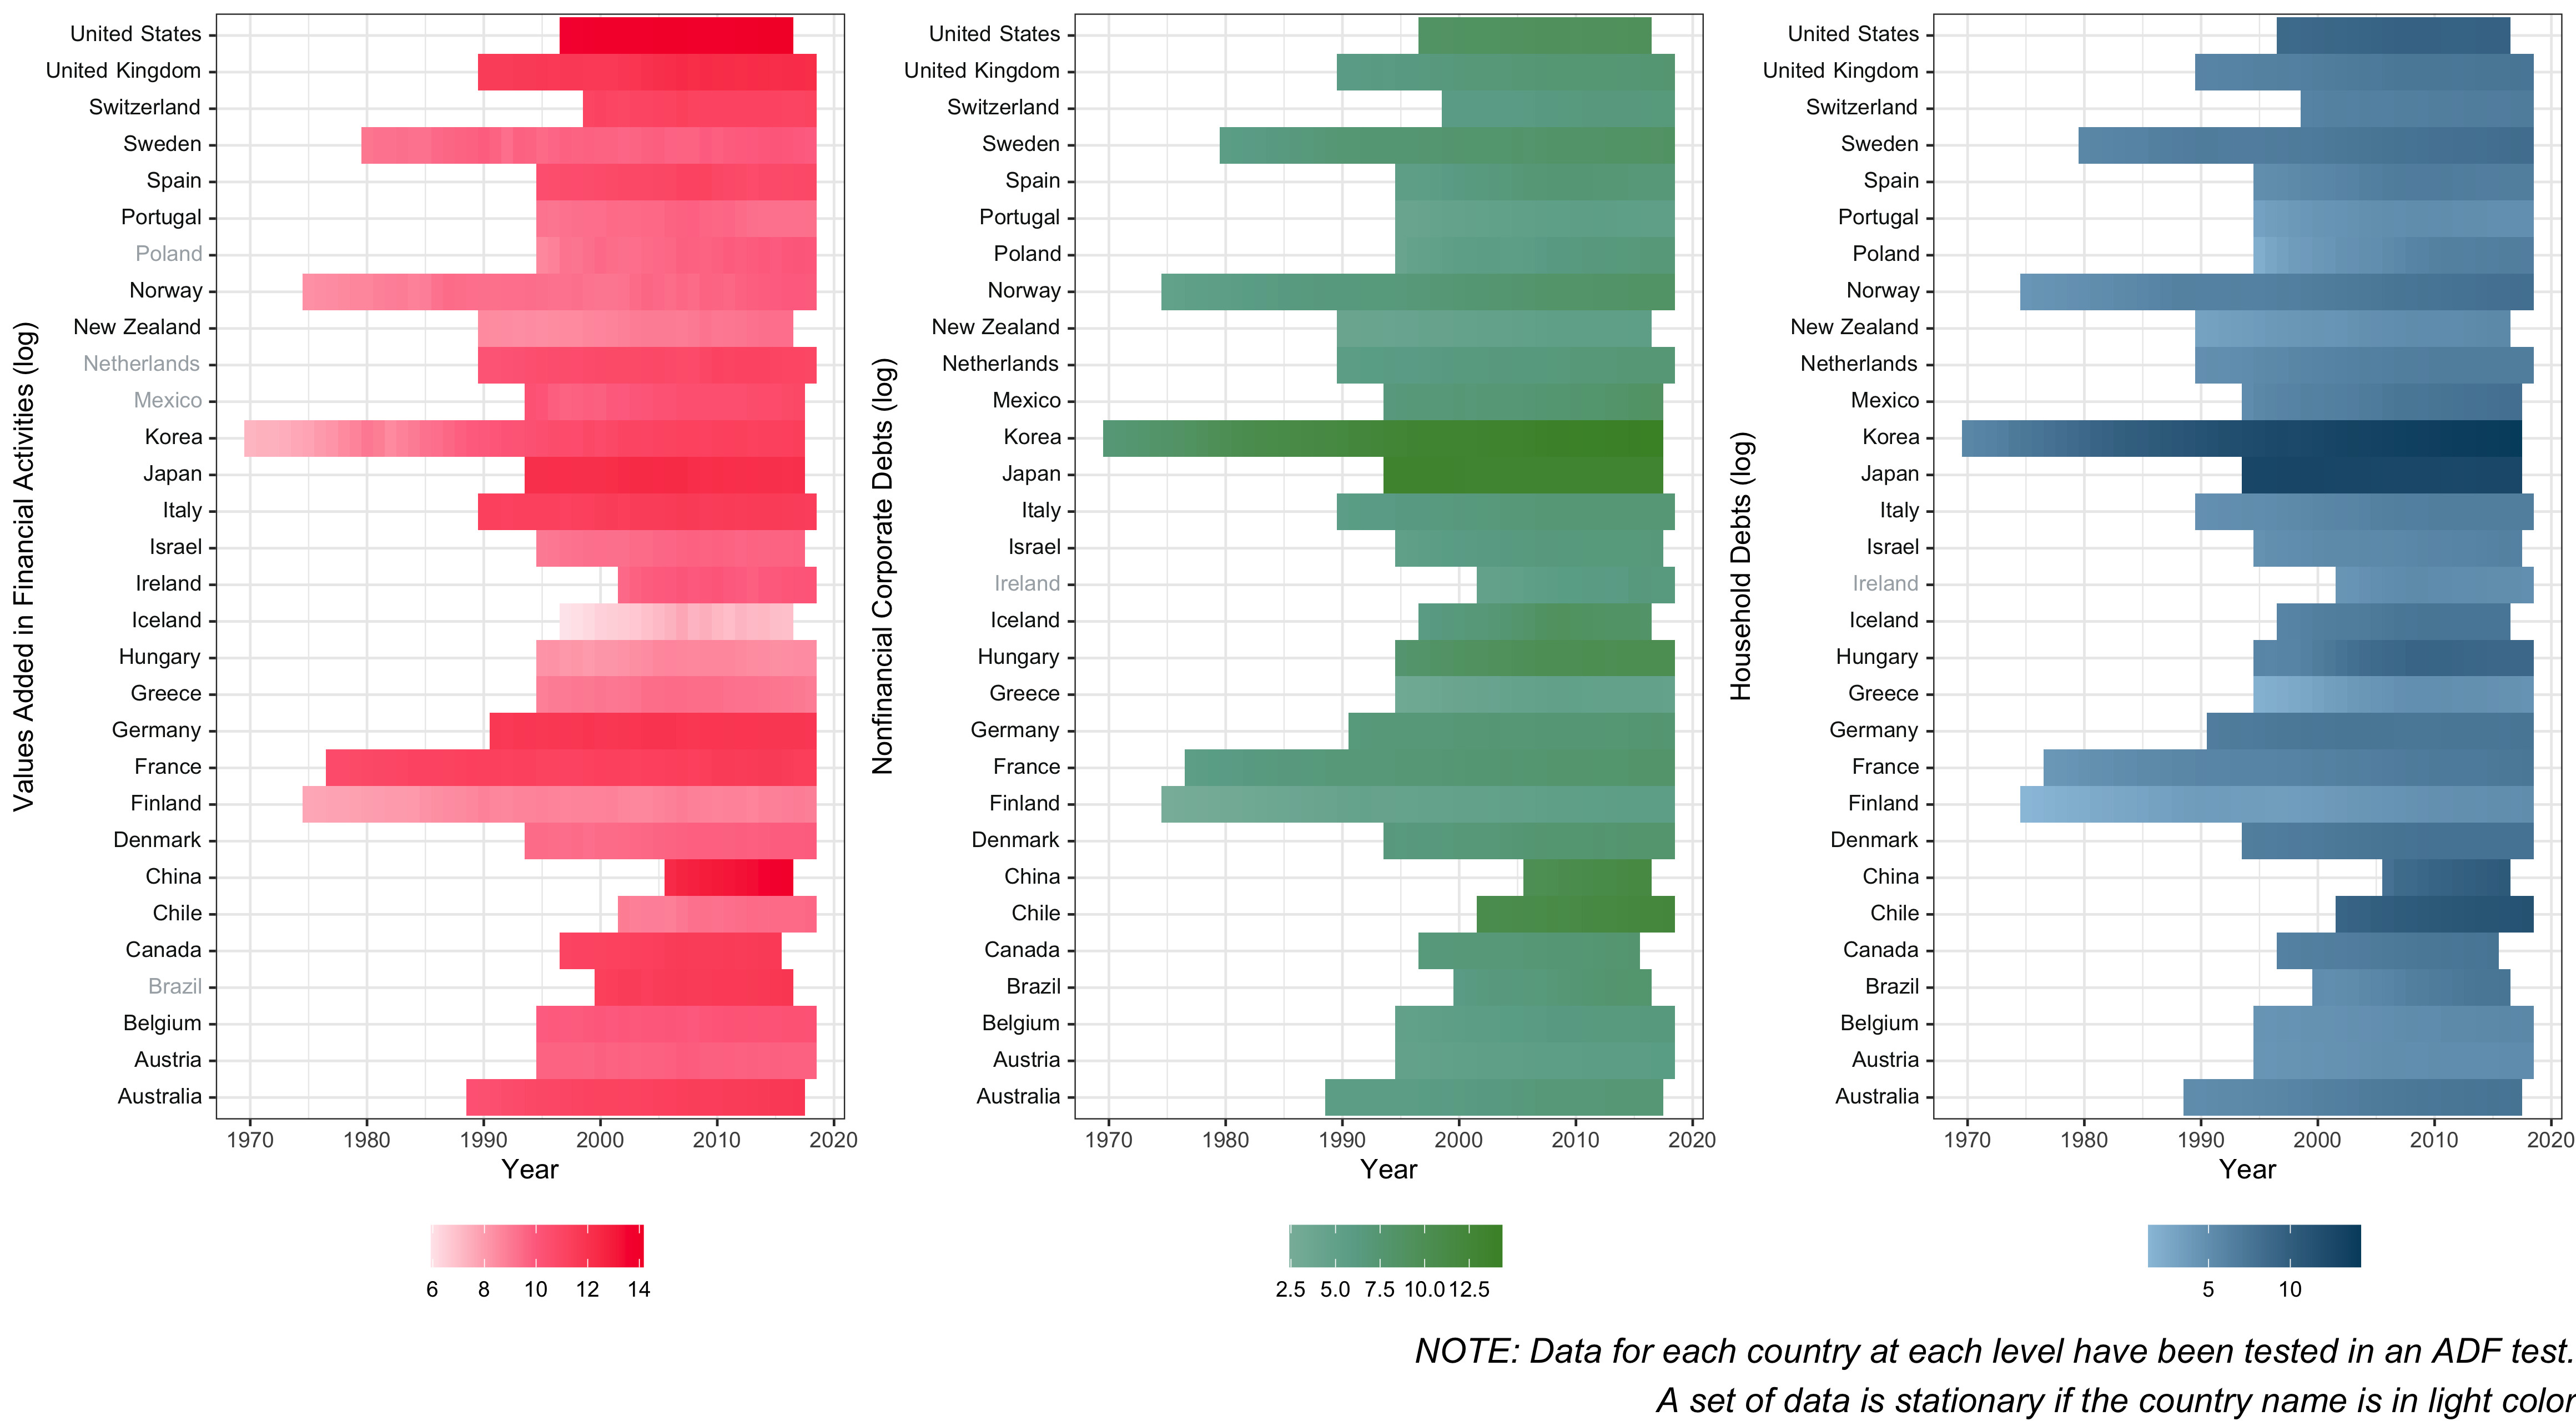
\includegraphics[width=64.44in,height=0.4\textheight]{table_and_figure/figure1} \caption{Stationarity of Financialization Measures across 39 Countries}\label{fig:unnamed-chunk-1}
\end{figure}

\textit{Notes:} Dots denote cities with monitoring stations
under India's National Ambient Air Monitoring Programme
(NAAMP).  Geographical data are drawn from MIT's Geodata
Repository.
\end{figure}

\begin{figure}
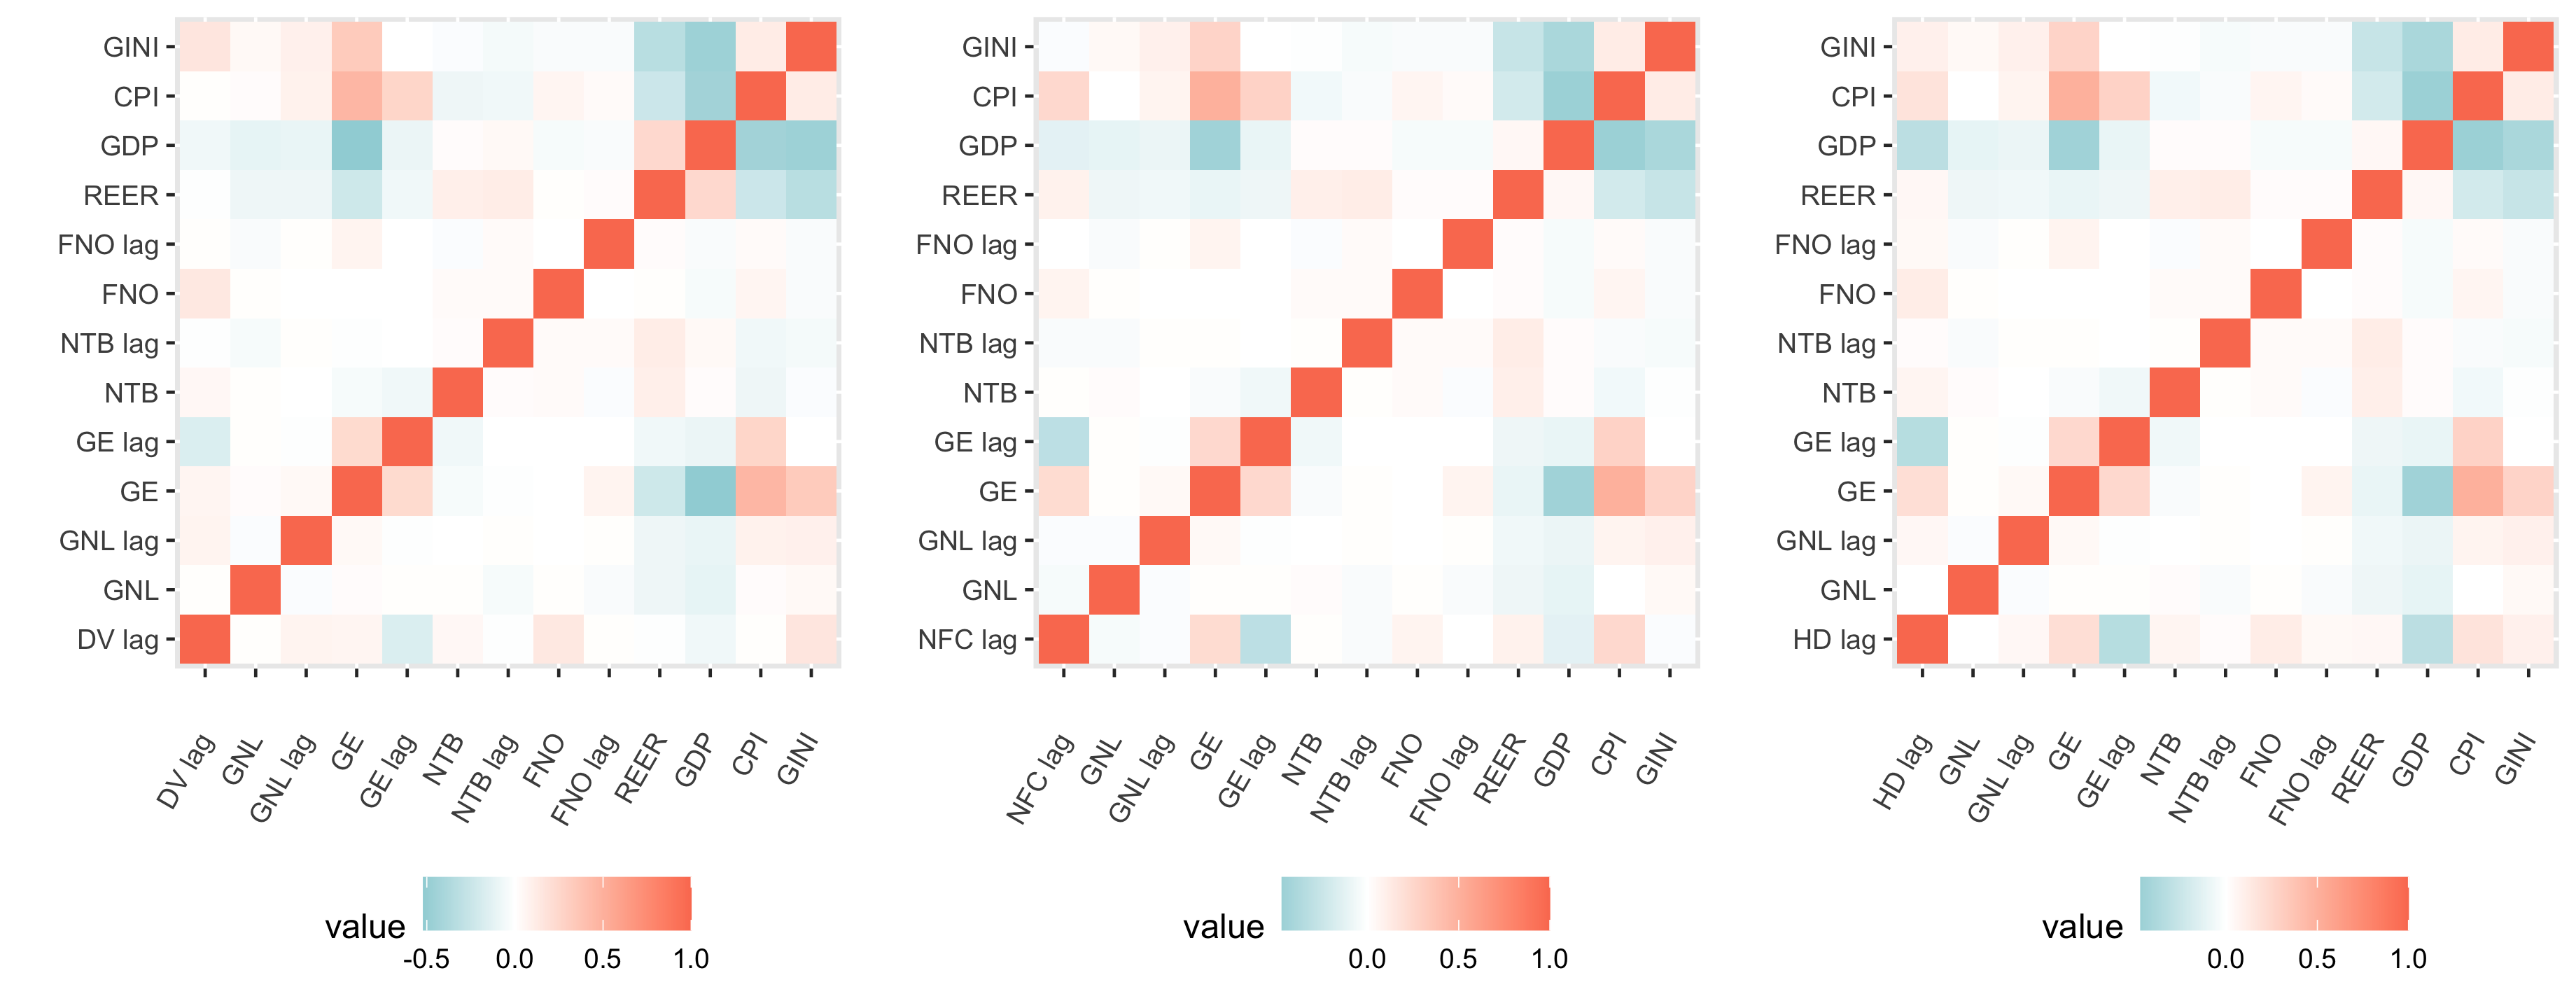
\includegraphics[width=51.11in,height=0.3\textheight]{table_and_figure/corf} \caption{Variable Correlations of The Three Models}\label{fig:ip}
\end{figure}

\begin{table}

\caption{\label{tab:unnamed-chunk-2}Model Selection Tests}
\centering
\begin{tabular}[t]{lrrr}
\toprule
 & Value Added & NFC debts & Household Debts\\
\midrule
\addlinespace[0.3em]
\multicolumn{4}{l}{\textbf{Breusch-Pagan LM test for cross-sectional dependence}}\\
\hspace{1em}Chi-square & 616.160 & 597.800 & 960.890\\
\hspace{1em}p-value & 0.000 & 0.000 & \vphantom{1} 0.000\\
\addlinespace[0.3em]
\multicolumn{4}{l}{\textbf{Breusch-Pagan test for heteroskadasticity}}\\
\hspace{1em}Breusch-Pagan & 263.110 & 410.620 & 1834.500\\
\hspace{1em}p-value & 0.000 & 0.000 & 0.000\\
\addlinespace[0.3em]
\multicolumn{4}{l}{\textbf{Breusch-Godfrey test for serial correlation}}\\
\hspace{1em}Lagrange Multiplier & 1.588 & 10.940 & 53.794\\
\hspace{1em}p-value & 0.208 & 0.001 & 0.000\\
\bottomrule
\end{tabular}
\end{table}

\begin{table}

\caption{\label{tab:unnamed-chunk-3}Dynamic Regression Models with Panel-Corrected Standard Errors, 1972-2012}
\centering
\begin{tabular}[t]{lccc}
\toprule
  & M1: Values added & M2: NFC debts & M3: Household debts\\
\midrule
(Intercept) & -0.002 & -0.259** & -0.093\\
 & (0.170) & (0.121) & (0.145)\\
Dependent variable (lag 1) & 0.019 & 0.138*** & 0.018\\
 & (0.022) & (0.037) & (0.036)\\
\addlinespace[0.3em]
\multicolumn{4}{l}{\textbf{Statecraft contigency}}\\
\hspace{1em}Government net lending & -0.001 & -0.002** & -0.001\\
\hspace{1em} & (0.001) & (0.001) & \vphantom{1} (0.001)\\
\hspace{1em}Government net lending (lag 1) & -0.002* & -0.002*** & -0.002*\\
\hspace{1em} & (0.001) & (0.001) & (0.001)\\
\hspace{1em}Government expenditure & 0.399*** & 0.061 & 0.164\\
\hspace{1em} & (0.113) & (0.096) & (0.115)\\
\hspace{1em}Government expenditure (lag 1) & 0.000 & 0.000*** & 0.000***\\
\hspace{1em} & (0.000) & (0.000) & \vphantom{3} (0.000)\\
\addlinespace[0.3em]
\multicolumn{4}{l}{\textbf{Development pitfall}}\\
\hspace{1em}Net trade balance & 0.000 & -0.001 & 0.003\\
\hspace{1em} & (0.002) & (0.002) & \vphantom{2} (0.002)\\
\hspace{1em}Net trade balance (lag 1) & 0.001 & 0.001 & 0.000\\
\hspace{1em} & (0.002) & (0.002) & \vphantom{1} (0.002)\\
\hspace{1em}FDI net outflows & 0.000 & 0.000 & 0.000\\
\hspace{1em} & (0.000) & (0.000) & \vphantom{2} (0.000)\\
\hspace{1em}FDI net outflows (lag1) & 0.000 & 0.000 & 0.000\\
\hspace{1em} & (0.000) & (0.000) & \vphantom{1} (0.000)\\
\addlinespace[0.3em]
\multicolumn{4}{l}{\textbf{Control variable}}\\
\hspace{1em}Real Effect Exchange Rates & 0.001 & 0.002*** & 0.001\\
\hspace{1em} & (0.001) & (0.000) & (0.001)\\
\hspace{1em}GDP & 0.000 & 0.000** & 0.000**\\
\hspace{1em} & (0.000) & (0.000) & (0.000)\\
\hspace{1em}CPI & 0.000 & 0.007*** & -0.002\\
\hspace{1em} & (0.002) & (0.002) & (0.003)\\
\hspace{1em}GINI & 0.000 & 0.001 & 0.002\\
\hspace{1em} & (0.002) & (0.002) & (0.002)\\
\midrule
Num.Obs. & 405 & 417 & 417\\
R2 & 0.333 & 0.581 & 0.630\\
R2 Adj. & 0.184 & 0.478 & 0.540\\
AIC & -777.7 & -959.7 & -809.6\\
BIC & -473.4 & -620.9 & -470.8\\
Log.Lik. & 464.871 & 563.844 & 488.807\\
F & 2.227 & 5.646 & 6.950\\
\bottomrule
\multicolumn{4}{l}{\textsuperscript{} * p $<$ 0.1, ** p $<$ 0.05, *** p $<$ 0.01}\\
\end{tabular}
\end{table}

\begin{table}

\caption{\label{tab:unnamed-chunk-4}Error Correction Models, 1972-2012}
\centering
\begin{tabular}[t]{lccc}
\toprule
  & M4: Values added & M5: NFC debts & M6: Household debts\\
\midrule
(Intercept) & 0.114* & -0.044 & 0.250***\\
 & (0.063) & (0.059) & (0.072)\\
\addlinespace[0.3em]
\multicolumn{4}{l}{\textbf{Statecraft contigency}}\\
\hspace{1em}Government net lending & -0.001 & -0.003** & 0.000\\
\hspace{1em} & (0.001) & (0.001) & \vphantom{1} (0.001)\\
\hspace{1em}Government net lending (lag 1) & -0.003* & -0.005*** & -0.003\\
\hspace{1em} & (0.002) & (0.002) & \vphantom{2} (0.002)\\
\hspace{1em}Government expenditure & 0.354*** & 0.222*** & 0.401***\\
\hspace{1em} & (0.095) & (0.085) & (0.102)\\
\hspace{1em}Government expenditure (lag 1) & 0.378*** & 0.242** & 0.328**\\
\hspace{1em} & (0.122) & (0.115) & (0.138)\\
\addlinespace[0.3em]
\multicolumn{4}{l}{\textbf{Development pitfall}}\\
\hspace{1em}Net trade balance & -0.001 & 0.000 & 0.001\\
\hspace{1em} & (0.002) & (0.002) & \vphantom{1} (0.002)\\
\hspace{1em}Net trade balance (lag 1) & 0.001 & 0.001 & 0.002\\
\hspace{1em} & (0.003) & (0.002) & (0.003)\\
\hspace{1em}FDI net outflows & 0.000 & 0.000 & 0.000\\
\hspace{1em} & (0.000) & (0.000) & \vphantom{2} (0.000)\\
\hspace{1em}FDI net outflows (lag1) & 0.000 & 0.000 & 0.000\\
\hspace{1em} & (0.000) & (0.000) & \vphantom{1} (0.000)\\
\addlinespace[0.3em]
\multicolumn{4}{l}{\textbf{Control variable}}\\
\hspace{1em}Real Effect Exchange Rates & 0.000 & 0.001* & 0.000\\
\hspace{1em} & (0.001) & (0.001) & (0.001)\\
\hspace{1em}GDP & 0.000 & 0.000 & 0.000***\\
\hspace{1em} & (0.000) & (0.000) & (0.000)\\
\hspace{1em}CPI & 0.000 & 0.015*** & 0.002\\
\hspace{1em} & (0.002) & (0.002) & (0.002)\\
\hspace{1em}GINI & 0.000 & 0.002* & -0.003**\\
\hspace{1em} & (0.002) & (0.001) & (0.002)\\
\midrule
Num.Obs. & 404 & 416 & 416\\
R2 & 0.509 & 0.441 & 0.415\\
R2 Adj. & 0.487 & 0.417 & 0.390\\
AIC & -772.3 & -926.1 & -775.8\\
BIC & -696.3 & -849.6 & -699.2\\
Log.Lik. & 405.149 & 482.072 & 406.884\\
F & 23.510 & 18.444 & 16.603\\
\bottomrule
\multicolumn{4}{l}{\textsuperscript{} * p $<$ 0.1, ** p $<$ 0.05, *** p $<$ 0.01}\\
\end{tabular}
\end{table}

\end{document}
